\documentclass[landscape,a4paper,9pt]{extarticle}
\usepackage[utf8x]{inputenc}
\usepackage[ngerman]{babel}
\usepackage[T1]{fontenc}
\usepackage{tikz}
\usetikzlibrary{shapes,positioning,arrows,fit,calc,graphs,graphs.standard}
\usepackage[nosf]{kpfonts}
\usepackage[t1]{sourcesanspro}
\usepackage{multicol}
\usepackage{wrapfig}
\usepackage[top=5mm,bottom=5mm,left=5mm,right=5mm]{geometry}
\usepackage[framemethod=tikz]{mdframed}
\usepackage{microtype}
\usepackage{pdfpages}

\usepackage{graphicx}
\graphicspath{ {./img/} }
\usepackage{minted} % for code blocks

\let\bar\overline

\definecolor{myblue}{cmyk}{1,.72,0,.38}
\definecolor{myheaderblue}{cmyk}{75, .50, 0, .50}
\definecolor{mathcolor}{cmyk}{100, 0, .50, .25}

\def\firstcircle{(0,0) circle (1.5cm)}
\def\secondcircle{(0:2cm) circle (1.5cm)}

\colorlet{circle edge}{myblue}
\colorlet{circle area}{myblue!5}

\tikzset{filled/.style={fill=circle area, draw=circle edge, thick},
    outline/.style={draw=circle edge, thick}}
    
\pgfdeclarelayer{background}
\pgfsetlayers{background,main}

\everymath\expandafter{\the\everymath \color{mathcolor}}
\everydisplay\expandafter{\the\everydisplay \color{myblue}}

\renewcommand{\baselinestretch}{.4}
\pagestyle{empty}

\global\mdfdefinestyle{header}{%
linecolor=gray,linewidth=1pt,%
leftmargin=0mm,rightmargin=0mm,skipbelow=0mm,skipabove=0mm,
}

\newcommand{\header}{
\begin{mdframed}[style=header]
\footnotesize
\sffamily
21 Karp Probleme ~Seite~\thepage~von~2 \\
~Janosch~Bühler und Ismael Embaby
\end{mdframed}
}

\makeatletter % Author: https://tex.stackexchange.com/questions/218587/how-to-set-one-header-for-each-page-using-multicols
\renewcommand{\section}{\@startsection{section}{1}{0mm}%
                                {.2ex}%
                                {.2ex}%x
                                {\color{myheaderblue}\sffamily\small\bfseries}}
\renewcommand{\subsection}{\@startsection{subsection}{1}{0mm}%
                                {.2ex}%
                                {.2ex}%x
                                {\sffamily\bfseries}}



\def\multi@column@out{%
   \ifnum\outputpenalty <-\@M
   \speci@ls \else
   \ifvoid\colbreak@box\else
     \mult@info\@ne{Re-adding forced
               break(s) for splitting}%
     \setbox\@cclv\vbox{%
        \unvbox\colbreak@box
        \penalty-\@Mv\unvbox\@cclv}%
   \fi
   \splittopskip\topskip
   \splitmaxdepth\maxdepth
   \dimen@\@colroom
   \divide\skip\footins\col@number
   \ifvoid\footins \else
      \leave@mult@footins
   \fi
   \let\ifshr@kingsaved\ifshr@king
   \ifvbox \@kludgeins
     \advance \dimen@ -\ht\@kludgeins
     \ifdim \wd\@kludgeins>\z@
        \shr@nkingtrue
     \fi
   \fi
   \process@cols\mult@gfirstbox{%
%%%%% START CHANGE
\ifnum\count@=\numexpr\mult@rightbox+2\relax
          \setbox\count@\vsplit\@cclv to \dimexpr \dimen@-1cm\relax
\setbox\count@\vbox to \dimen@{\vbox to 1cm{\header}\unvbox\count@\vss}%
\else
      \setbox\count@\vsplit\@cclv to \dimen@
\fi
%%%%% END CHANGE
            \set@keptmarks
            \setbox\count@
                 \vbox to\dimen@
                  {\unvbox\count@
                   \remove@discardable@items
                   \ifshr@nking\vfill\fi}%
           }%
   \setbox\mult@rightbox
       \vsplit\@cclv to\dimen@
   \set@keptmarks
   \setbox\mult@rightbox\vbox to\dimen@
          {\unvbox\mult@rightbox
           \remove@discardable@items
           \ifshr@nking\vfill\fi}%
   \let\ifshr@king\ifshr@kingsaved
   \ifvoid\@cclv \else
       \unvbox\@cclv
       \ifnum\outputpenalty=\@M
       \else
          \penalty\outputpenalty
       \fi
       \ifvoid\footins\else
         \PackageWarning{multicol}%
          {I moved some lines to
           the next page.\MessageBreak
           Footnotes on page
           \thepage\space might be wrong}%
       \fi
       \ifnum \c@tracingmulticols>\thr@@
                    \hrule\allowbreak \fi
   \fi
   \ifx\@empty\kept@firstmark
      \let\firstmark\kept@topmark
      \let\botmark\kept@topmark
   \else
      \let\firstmark\kept@firstmark
      \let\botmark\kept@botmark
   \fi
   \let\topmark\kept@topmark
   \mult@info\tw@
        {Use kept top mark:\MessageBreak
          \meaning\kept@topmark
         \MessageBreak
         Use kept first mark:\MessageBreak
          \meaning\kept@firstmark
        \MessageBreak
         Use kept bot mark:\MessageBreak
          \meaning\kept@botmark
        \MessageBreak
         Produce first mark:\MessageBreak
          \meaning\firstmark
        \MessageBreak
        Produce bot mark:\MessageBreak
          \meaning\botmark
         \@gobbletwo}%
   \setbox\@cclv\vbox{\unvbox\partial@page
                      \page@sofar}%
   \@makecol\@outputpage
     \global\let\kept@topmark\botmark
     \global\let\kept@firstmark\@empty
     \global\let\kept@botmark\@empty
     \mult@info\tw@
        {(Re)Init top mark:\MessageBreak
         \meaning\kept@topmark
         \@gobbletwo}%
   \global\@colroom\@colht
   \global \@mparbottom \z@
   \process@deferreds
   \@whilesw\if@fcolmade\fi{\@outputpage
      \global\@colroom\@colht
      \process@deferreds}%
   \mult@info\@ne
     {Colroom:\MessageBreak
      \the\@colht\space
              after float space removed
              = \the\@colroom \@gobble}%
    \set@mult@vsize \global
  \fi}

\makeatother
\setlength{\parindent}{0pt}

\begin{document}
\footnotesize
\begin{multicols*}{5}
\section{Vorgehen}
\begin{enumerate}
\item Gewähltes Problem aus dem Katalog von Karp notieren
\item Reduktion des gegebenen Problems, auf das bekannte aus Karp
\item Beschreibung der Reduktion
\item Schlussfolgerung: Da das Problem aus dem Katalog von Karp NP-vollständig ist, gibt es auch keinen effizienten (polynomiellen) Algorithmus, der das gegebene Problem lösen könnte.
\end{enumerate}
Schlusssatz:
Dies ist genau die Beschreibung des Problems HMMM. Das Problem HMMM ist NP-vollständig, nach aktuellem Wissen gibt es also keinen effizienten (polynomiellen) Algorithmus, der ein HMMM Problem lösen könnte.

Manchmal ist es schwierig SET-COVERING, EXACT-COVER und SET-PACKING auseinander
zu halten. Man beachte:
- In SET-COVERING und in SET-PACKING kommt eine Zahl k vor, nicht aber in EXACT-
COVER.
- In SET-COVERING dürfen sich die Mengen schneiden, müssen aber auch alles abdecken.
In SET-PACKING dürfen sich die Mengen nicht schneiden, müssen aber auch nicht alles
abdecken.
- In EXACT-COVER dürfen sich die Mengen nicht schneiden, müssen alles abdecken, aber
es kommt nicht auf ihre Anzahl an.

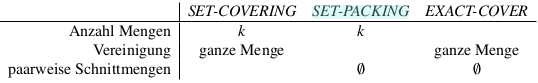
\includegraphics[width=\columnwidth]{img/setvscoveringvsexact.png}
\section{3D-Matching}
\subsection{Konzertprogramm}
Ein Orchester soll Konzertprogramme für eine Saison zusammenstellen. Zur Verfügung steht eine Menge von Werken, die das Orchester im Repertoire hat. Aus diesen Werken sollen Programme mit jeweils drei Werken zusammengesetzt werden. Je ein Werk zur Eröffnung, für den Mittelteil und zum Abschluss des Konzertes. Die Werke lassen sich nicht beliebig kombi- nieren, weil zum Beispiel die Tonarten nicht zu verschieden sein dürfen. Die Anzahl der Werke und der Konzertabende der Saison ist gleich. Es stellt sich heraus, dass es ziemlich schwierig ist, Programme so zu konstruieren, dass kein Werk in der gleichen Phase eines Konzerts mehr als einmal gespielt wird. Warum?\\
\\
\textbf{Lösung}
Dies ist eine Instanz des 3D-Matching-Problems. Die Menge der Werke ist T , die Menge der möglichen Programme (Einschränkungen zum Beispiel durch Tonart) ist U ⊂ T × T × T . Gesucht werden solle eine Menge von Programmen W ⊂ U, mit |W| = |T |, so dass keine zwei Elemente in irgend einer Koordinate übereinstimmen. Da 3D-Matching NP-vollständig ist, ist auch das Konzertproblem NP-vollständig, nach aktuellem Wissen gibt es dafür daher keinen polynomiellen Algorithmus.
\subsection{Rezepte}
Ein Koch hat je n Rezepte für Vorspeisen, Hauptspeisen und Desserts. Nicht alle Vorspeisen lassen sich mit jeder Hauptspeise kombinieren, dasselbe gilt auch für Desserts. Damit jedes seiner Rezepte regelmässig zum Einsatz kommt, möchte der Koch eine Folge von n Menus zusammenstellen, so dass jedes Rezept in genau einem der Menus vorkommt. Nach längerem tüfteln gibt er jedoch frustriert auf. Können Sie erklären, warum ihm die Menugestaltung so schwer gefallen ist.\\
\\
\textbf{Lösung}
Es handelt sich hier um das Problem 3D-MATCHING. Die Menge T sind die Nummern der Rezepte, die Tripel aus 
T × T × T sind die Menuzusammenstellungen, bestehend aus je einer Nummer für ein Vorspeisen-, ein Hauptspeisen- und ein Dessert-Rezept. Die Menge U ist die Menge der möglichen Menukombinationen. Die gesuchte Teilmenge W ist eine Auswahl von n = |T | = |W| Menus derart, dass keine Vorspeise (erste Komponente), keine Hauptspeise (zweite Komponente) und kein Dessert (dritte Komponente) mehr als einmal vorkommt. Das Problem 3D-MATCHING ist NP-vollständig, es ist daher kein Algorithmus bekannt, der das Problem in polynomieller Zeit lösen könnte.
\section{Clique-Cover}
\subsection{Gruppenarbeit}
Für eine Gruppenarbeit sollen k Gruppen gebildet werden. Um die Zeit für das gegen- seitige Kennenlernen möglichst kurz zu halten, sollen sich die Leute einer Gruppe bereits ge- genseitig kennen. Alle Leute sollen beschäftigt sein. Können Sie einen effizienten Algorithmus formulieren, mit dem eine solche Gruppeneinteilung auch bei einer grossen Teilnehmerzahl gefunden werden kann?\\
\\
\textbf{Lösung}
Das Problem ist äquivalent zu CLIQUE-COVER, also NP-vollständig. Nach aktuellem Wissen gibt es also keine effizienten Algorithmus, der das Problem lösen würde. Die Äquivalenz wird durch folgende Abbildung vermittelt\\
Teilnehmer $\rightarrow$ Knoten\\
kenne sich $\rightarrow$ Kante\\
Anzahl Gruppen $\rightarrow$ k\\
Gruppe $\rightarrow$ Clique\\

\section{Exact-Cover}
\subsection{Kundenanalyse}
Student Xaver Tecco soll im Rahmen einer Big-Data-Studienarbeit die Kunden einer gros- sen Shop-Website untersuchen und klassifizieren. Es steht eine grosse Zahl von binären Eigen- schaften zur Verfügung, zum Beispiel ob Kunden ein bestimmtes Produkt gekauft haben, oder ob ein Kunde nur im Dezember einkauft. Herr Tecco soll herausfinden, ob es eine Teilmenge von Kriterien derart gibt, dass jeder Kunde genau eine der Eigenschaften hat. Die Abgabe der Arbeit steht in zwei Tagen bevor, und er hat noch keinen funktionierenden Algorithmus. Muss er sich Sorgen machen?\\
\\
\textbf{Lösung}
Dieses Problem ist äquivalent mit dem bekanntermassen NP-vollständigen Problem EXACT-COVER:
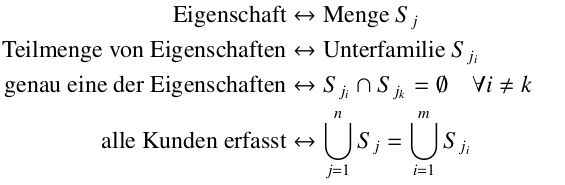
\includegraphics[width=\columnwidth]{img/exact-cover.png}

\subsection{Sehenswürdigkeiten}
Ein Tourist besucht ein fernes Land und kauft sich bei der Ankunft am Flughafen einen Führer, der all die zahlreichen Sehenswürdigkeiten enthält, die er gerne besuchen möchte. Er sagt sich, dass er seine Besichtigungspläne am besten so organisiert, dass er an jedem Tag eine Gruppe von Sehenswürdigkeiten besucht, die nahe beeinander liegen. Als nahe beeinander liegend klassifiziert er jeweils solche, die in kurzer Zeit mit öffentlichen Verkehrsmitteln erreichbar sind. Für jeden Tag seines Aufenthalts könnte er dann genau eine Gruppe von Sehenswürdig- keiten auswählen, so dass er am Ende alle gewünschten Sehenswürdigkeiten gesehen hat und keine zweimal besucht. Dank eines Sabbaticals war er zeitlich frei und stellte sich vor, seinen Aufenhalt nötigenfalls zu verlängern, sollte er mit seinen Besichtigungen nicht durchkommen. Nach einigen fehlgeschlagenen Versuchen, das Problem im Kopf zu lösen, setzt er sich in eine Caffeteria am Flughafen und arbeitet an dem Problem weiter. Er sagt sich, dass eine sorgfältige Planung durchaus einen ersten Tag ohne Besuch einer Sehenswürdigkeit wert ist. Als es dunkel wird ohne dass er eine Lösung gefunden hat, muss er sich eingestehen, dass das Problem doch nicht ganz einfach ist und beschliesst, am nächsten Morgen weiterzuarbeiten. Schliesslich geht nichts über eine sorgfältige Planung. Warum besteht die Gefahr, dass der arme Mann seine Heimreise antreten wird, ohne auch nur eine einzige Sehenswürdigkeit besucht zu haben?\\
\\
\textbf{Lösung}
Das beschriebene Problem BESICHTIGUNGS-PLANUNG ist das NP-vollständige Problem EXACT-COVER, für das es nach aktuellem Wissen keinen polynomiellen Algorithmus gibt. Die Menge U besteht aus allen Sehenswürdigkeiten des Führers. Die Teilmengen S j sind die Sehenswürdigkeiten, die der Tourist als nahe beeinander klassifiziert hat. Die Vereinigung $\bigcup_{j=1}^n S_j$ umfasst die Sehenswürdigkeiten, die der Tourist in seine Planung einbezogen hat. Gesucht ist eine disjunkte Teilfamilie $S_{j_i}$ , die alle Sehenswürdigkeiten umfasst, also
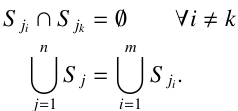
\includegraphics[width=\columnwidth/2]{img/sehenswuerdigkeiten.png}
\section{Feedback-Arc-Set}
\subsection{COVID-19 Sicherheitsmassnahmen}
Die COVID-19 Pandemie verlangt von Läden Sicherheitsmassnahmen, die sicherstellen sollen, dass die Kunden in sicheren Abständen verbleiben. Ein Einkaufszentrum entscheidet daher, dass ein Einbahnbetrieb eingeführt werden soll. Die Marketing-Abteilung legt fest, in welcher Richtung die einzelnen Gänge zwischen den Gestellen durchlaufen werden können sollen. Es soll nämlich sichergestellt werden, dass die Kunden immer noch in der “richtigen” Reihenfolge mit überflüssiger Werbung zu genauso überflüssigen Spontankäufen verleitet werden sollen. Schliesslich will der Sicherheitsverantwortliche wissen, ob es möglich ist, in einigen Gängen Desinfektionsstationen aufzustellen so, dass jeder Kunde, der sich auf einem geschlossenen Weg durch das Einkaufszentrum bewegt, mindestens einmal an einer Desinfektionsstation vorbeikommt. Dabei dürfen nicht mehr Desinfektionsstationen verwendet werden, als das vorgegebene Budget erlaubt. Dies stürtzt die Planer in eine Krise, auch nach stundenlangem Probieren können Sie keine definitive Antwort geben. Warum?\\
\\
\textbf{Lösung}
Das beschriebene Problem ist das Problem FEEDBACK-ARC-SET, wie die folgenden
Eins-zu-eins-Reduktion zeigt:\\
Graph $\leftrightarrow$ Plan des Einkaufszentrums\\
Knoten $\leftrightarrow$ Kreuzungsstellen\\
Kanten $\leftrightarrow$ Gänge\\
Richtung $\leftrightarrow$ Einbahnrichtung in jedem Gang\\
Anzahl k $\leftrightarrow$ Budget für Desinfektionsstationen\\
Arc set $\leftrightarrow$ Platzierung der Desinfektionsstationen
\section{Feedback-Node-Set}
Gleiche Aufgabe wie oben aber leicht andere Lösung\\
\\
\textbf{Lösung}
Das beschriebene Problem ist das Problem FEEDBACK-NODE-SET, wie die folgen-
den Eins-zu-eins-Reduktion zeigt:\\
Graph $\leftrightarrow$ Plan des Einkaufszentrums\\
Knoten $\leftrightarrow$ Kreuzungsstellen\\
Kanten $\leftrightarrow$ Gänge\\
Richtung $\leftrightarrow$ Einbahnrichtung in jedem Gang\\
Anzahl k $\leftrightarrow$ Budget für Desinfektionsstationen\\
Node set $\leftrightarrow$ Platzierung der Desinfektionsstationen\\
\section{Hitting-Set}
\subsection{Expertenkomission}
Aus einer Menge von Fachleuten, die zum Teil in mehreren Gebieten i = 1, . . . , n tätig sind, soll eine Expertenkommission gebildet werden. Da zwei Experten für das gleiche Fachgebiet sich erfahrungsgemäss immer streiten, will man in der Expertenkommission jedes Fachgebiet durch genau einen Experten vertreten haben. Können Sie einen effizienten Algorithmus zur Auswahl der Mitglieder der Kommission angeben?\\
\\
\textbf{Lösung}
Das Problem ist Äquivalent zu HITTING-SET, ist also NP-vollständig. Nach aktuellem Wissen gibt es also keine effizienten Algorithmus, der das Problem lösen würde. Die Äquivalenz zu HITTING-SET wird durch die Abbildung vermittelt\\
\\
Experte $\rightarrow$ Punkt in S\\
Fachgebiet i $\rightarrow$ Teilmenge $U_i$ aller Experten für dieses Gebiet\\
Expertenkommission $\rightarrow$ Hitting Set H\\

\subsection{Landesbewohner gruppieren}
Die Bewohner eines Landes lassen sich nach einer grossen Zahl von Kriterien in Gruppen einteilen: nach Berufsgruppen, nach Altersgruppen, nach kulturellen Interessen, nach Hobbies usw. Jetzt soll eine Interessenvertretung gebildet werden so, dass jede dieser Gruppen mit genau einem Mitglied vertreten ist. Dabei ist es durchaus zulässig, dass die Gruppe der Raketenmodellbauer und die Gruppe der Freunde von Kammermusik von der gleichen Person vertreten werden. Aber es darf nicht sein, dass sich der Vertreter der Astrophotographen auch noch für Kammermusik interessiert, denn dann hätten die Kammermusikfreunde zwei Vertreter. Gibt es einen effizienten Algorithmus, der auch bei einer grossen Zahl von Bewohnern und Gruppierungen entscheiden kann, ob eine solche Zusammenstellung einer Interessenvertretung überhaupt möglich ist?\\
\\
\textbf{Lösung}
Nein, denn das Problem ist NP-vollständig, wie wir gleich zeigen werden, nach unserem aktuellen Wissen also höchstwahrscheinlich nicht mit einem effizienten Algorithmus lösbar. Und gäbe es einen effizienten Algorithmus, würde dies automatisch P = NP zur Folge haben. Seien die $i$ $\in$ $I$ die Kriterien, nach denen gruppiert wird, und sei $S_i$ die Menge der Bewohner,S die zur Gruppe i gehört. Gesucht wird jetzt ein Teilmenge H $\subset$ $\bigcup_{i \in I} S_i$ von Interessenvertretern so, dass H mit jeder der Mengen S i genau einen Vertreter gemeinsam hat: |H $\cap$ S i | = 1 für alle i. Dies ist das Problem HITTING-SET.\\

\subsection{Teambildung}
Ein etwas unerfahrener Event-Manager hat sich für seinen nächsten Event ein Spiel einfallen lassen, für das er die Gäste in Teams mit jeweils drei Mitgliedern einteilen muss. Damit die Bildung der Teams schnell vonstatten gehen kann, schickt er den Teilnehmern die Team-Nummer bereits mit der Einladung. Dummerweise lässt die Datenqualität seiner Adressdatenbank sehr zu wünschen übrig. Die meisten Teilnehmer bekommen mehrere Einladungen, mit verschiedenen Team-Nummern. Am Event kommt es zum Eklat. Der Manager versucht die Situation noch zu retten, indem er den Teilnehmern sagt, sie sollen die Dreierteams einfach mit einer der Teamnummern bilden, mit welcher spiele keine Rolle. Die Teilnehmer finden jedoch keine Lösung, der Event platzt, einige Teilnehmer gehen frühzeitig nach Hause, andere ersäufen ihren Frust an der Bar. Warum ist es so schwierig, nach Anweisung des Managers Teams zubilden?
\\
\textbf{Lösung}
Dieses Problem, welches wir TEAMBILDUNG nennen wollen, ist NP-vollständig, wie wir durch Vergleich mit dem bekanntermassen NP-vollständigen Problem EXACT-COVER nachweisen wollen. Je der vom Manager verschickten Nummern j definiert eine Teilmenge $S_j$ der Menge aller Teilnehmer U. Gesucht ist eine Unterfamilie Teams S j i , 1 ≤ i ≤ m, so dass keine zwei Teams sich überschneiden (d. h. kein Teilnehmer ist in mehr als einem Team) und die ganze Menge U überdecken (d. h. jeder Teilnehmer ist in einem Team). \\
\\
Reduktion auf HITTING-SET: Dazu bildet man für jeden Teilnehmer i die Menge S i der Teams, für die Teilnehmer i vorgesehen ist. Es ist klar, dass S i ⊂ S , wobei S die Menge aller Teams ist. Gesucht ist jetzt eine Auswahl von Teams so, dass jeder Teilnehmer in genau einem Team ist, also H ⊂ S so, dass |H ∩ S i | = 1. Das ist das Problem HITTING-SET.

\subsection{Selten bestiegene Gipfel}
Eine Zeitschrift für Alpinisten möchte eine Artikelserie über selten bestiegene Berggipfel veröffentlichen. Sie hat bereits eine Liste von Gipfeln zusammengestellt und bittet jetzt einen Alpinistenverein um eine Liste von Alpinisten als mögliche Interviewpartner, die über ihre Erfahrung beim Besteigen dieser Gipfel berichten können. Um Mehrspurigkeiten aus dem Weg zu gehen, soll kein Alpinist auf der Liste mehr als einen der aufgelisteten Gipfel bestiegen haben. Dem Verein fällt es sehr schwer, eine solche Liste zusammenzustellen, woran könnte das liegen?\\
\\
\textbf{Lösung}
Dies ist das Problem HITTING-SET. Die Liste der Gipfel ist die Menge I. Die Menge $S_i$ besteht aus allen Vereinsmitgliedern, die den Gipfel i bestiegen haben.\\
Liste der Gipfel ↔ I\\
Besteiger von Gipfel i ↔ S i\\
Alle in Frage kommenden Mitglieder ↔ S = $\bigcup_{i \in I} S_i$\\
\\
Ausgewählte Besteiger ↔ H

\subsection{Softwareentwicklungsprojekt}

Ein grosses Softwareentwicklungsprojekt ist wegen der aus dem Ruder gelaufenen Kosten.
gezwungen, zu redimensionieren. Zu diesem Zweck stellt der Projektleiter eine Liste von Skills
zusammen, die er nach der Entlassungswelle in seinem Team noch haben muss und kämpft nun
seit Tagen damit, ein Auswahl von Mitarbeitern zu finden, in der jeder Skill in genau einem
Teammitglied vertreten ist. Warum fällt ihm das so schwer?

Lösung. Dies ist das Problem HITTING-SET. Wir bezeichnen die Skills mit $i \in I, S_i$ ist die
Menge der Team-Mitglieder, die Skill $i$ haben. Gesucht ist eine Menge

$$H \subset \bigcup_{i\in I}S_i$$

derart, dass $|H \cap S_i| = 1$ für jeden Skill. Wir haben also eine 1-1-Reduktion

\begin{itemize}
\item Skills ↔ I
\item Skill ↔ i
\item Teammitglieder mit Skill i ↔ S i
\item neues Team ↔ H
\end{itemize}

Da HITTING-SET NP-vollständig ist, muss davon ausgegangen werden, dass es keinen Algo-
rithmus mit polynomieller Laufzeit zur Bestimmung der Menge H gibt. 
\section{Max-Cut}

Eine Firma konnte in einer feindlichen Übernahme einen wichtigen Konkurrenten aufkaufen. Der Konkurrent ist eigentlich eine Vereinigung von sehr vielen, sehr intensiv und effizient zusammenarbeitenden, aber im Übrigen weitgehend selbständigen Abteilungen, alle unter dem selben Dach. Das Ziel der Übernahme war, daraus die “Rosinen” herauszupicken, und den Rest zu schliessen. Die Wettbewerbsbehörden hatten dies vorausgesehen, und als Auflage für die Übernahme gemacht, dass keine einzige der Abteilungen geschlossen werden dürfe. Daher dachten sich die neuen Eigentümer den folgenden bösartigen Plan aus, um den gleichen Zweck zu erreichen. Sie teilten die Abteilungen auf zwei verschiedene Standorte auf, und sorgten dafür, dass jede Kommunikation zwischen den beiden Standorten so ineffizient wurde, dass die Abtei- lungen kaum mehr sinnvoll zusammenarbeiten konnten. Dadurch würden die einzelnen Abteilungen wirtschaftlich ruiniert, und man müsste sie trotz allem schliessen. Die neuen Eigentümer beauftragten daher eine Beratungsfirma, eine Aufteilung zu finden, mit der die Kommunikation zwischen den Abteilungen möglichst stark behindert würde. Die Beratungsfirma brauchte dafür sehr lange. Warum ist das nicht überraschend?

Es handelt sich hier um das Problem MAX-CUT. Wir beschreiben eine Reduktion des Problems auf MAX-CUT:

\begin{itemize}
\item Abteilung $\leftrightarrow$ Vertex
\item Kommunikationsbeziehung $\leftrightarrow$ Kante
\item Kommunikationsvolumen $\leftrightarrow$ Gewicht einer Kante
\end{itemize}

Die neuen Firmeneigentümer wollen die Menge der Vertices so in zwei Mengen aufteilen, dass die Summe der Gewichte der Kanten, die durch die Aufteilung zerschnitten werden, möglichst gross wird. Dies ist genau die Beschreibung des Problems MAX-CUT. Das Problem MAX-CUT ist NP-vollständig, nach aktuellem Wissen gibt es also keinen effizienten (polynomiellen) Algorithmus, der ein MAX-CUT Problem lösen könnte.
\section{Partition}

Ein aufstrebendes Film-Festival ist derart gewachsen, dass der Vorführsaal nicht mehr reicht. Daher müssen jetzt zwei gleich grosse Säle verwendet werden, und trotzdem ist das Festival wieder ausverkauft, und zwar in einem Masse, dass überhaupt nur Stars und Prominente samt ihrer Entourage eingelassen werden können, für einzelne Besucher gibt es keine Plätze. Doch die Stars stören sich daran, dass sie möglicherweise nicht ihre ganze Entourage im gleichen Saal haben können. Daher muss kurzfristig eine Aufteilung der Festival-Gäste gefunden werden, so dass die beiden Säle so gefüllt werden können, dass jede Entourage vollständig in einem der Säle Platz nimmt. Der Festival-Direktor ist jedoch sehr überrascht, dass die Bestimmung einer solchen Aufteilung so lange dauert. Warum sind Sie nicht überrascht?

\textbf{Lösung}. Zu jedem Star $i ∈ I$ gibt es eine Entourage mit $c_i$ Mitgliedern. Diese Menge muss jetzt
in zwei Teilmengen $A$ (Stars samt Entourage, die in Saal A Platz nehmen) und $B$ (Stars samt
Entourage, die in Saal B Platz nehmen) aufgeteilt werden, so dass $I = A ∪ B$. Die Aufteilung
muss so sein, dass in beiden Sälen gleich viele Leute Platz nehmen, also:

$$\Sigma_{i\in A} c_i = \Sigma_{i \in B} c_i$$


Dies ist das Problem PARTITION. Das gestellte Problem ist also äquivalent zum NP-vollständigen Problem PARTITION, und ist daher ebenfalls NP-vollständig. Man kann daher nach aktuellem Wissen nicht erwarten, dass es dafür einen effizienten Algorithmus gibt.
\section{Sequencing}

Die Prüfungsvorbereitungszeit ist intensiv, manchmal reicht die Zeit nicht, alle Prüfungen vorzubereiten, bis die Prüfungssession beginnt. Es ist daher unumgänglich, während der Prüfungssession weiter zu lernen. Nehmen wir an, dass für die Vorbereitung der $p$ Fächer $1,..., p$ die Vorbereitungszeiten $t_1 , ... , t_p$ notwendig sind. Ebenfalls bekannt ist, dass die Prüfungen zu den Zeiten $d_1 , . . . , d_p$ stattfinden, dann muss die Vorbereitung abgeschlossen sein, weil die Prüfung sonst nicht zu bestehen ist. Es stellt sich daher die Frage, in welcher Reihenfolge die Vorbereitungen durchgeführt werden sollen, damit höchstens k Prüfungen nicht bestanden werden. Ein Student, der AutoSpr nicht besucht hat, wendet viel Zeit dafür auf herauszufinden, ob es überheupt eine Reihenfolge dieser Art gibt, versteht aber nicht, warum dies so aufwendig ist. Können Sie dies erklären?

\textbf{Lösung}. Das vorliegende Problem ist das Problem SEQUENCING, welches bekanntermassen
NP-vollständig ist.

\begin{itemize}
\item Job $i$ $\leftrightarrow$ Vorbereitung für Fach $i$
\item Ausführungszeit $t_i$ $\leftrightarrow$ Vorbereitungszeit $t_i$
\item Deadline $d_i$ $\leftrightarrow$ Prüfungszeitpunkt $d_i$
\end{itemize}


Die Strafe für eine nicht bestandene Prüfung ist $s_1 = . . .= s_p = 1$, die Reihenfolge muss so gewählt werden, dass die Gesamtstrafe ≤ $k$ ist.
\section{Set-Covering}

Auf einem weit entfernten, aber technologisch sehr fortgeschrittenen Planeten wird der den Planeten regierende Ältestenrat nicht durch Volkswahl bestimmt, sondern durch einen Algorithmus. In der Vergangenheit gab es eine grosse Zahl rivalisierender Stämme, die sich auch zu grösseren “Nationen” verbündet haben und wiederholt blutige Kriege gegeneinander geführt haben. Um diesem Unheil ein Ende zu setzen, kamen die Stämme überein, den Ältestenrat zu bilden, in dem wenn auch nicht jeder Stamm direkt, so doch mindestens das “Blut” jedes Stammes vertreten sein musste. Damit trug man der Tatsache Rechnung, dass Mobiltät und planetenweiter Handel mittlerweile zu einer weitgehenden Durchmischung in der Bevölkerung geführt hatte. Ausgeprägtes Traditionsbewusstsein hatten jedoch sichergestellt, dass von jedem Bürger bekannt war, aus welchen Stämmen er “Blut” in sich trug. Warum ist trotzdem eine weit entwickelte Technologie nötig, um herauszufinden, ob sich ein Ältestenrat mit k Mitgliedern überhaupt bilden lässt?

Das Problem, einen Ältestenrat mit \textbf{k} Mitgliedern zu bilden, ist äquivalent zum Set-Covering Problem. Zu jedem Bürger \textbf{i} ist die Menge \textbf{$S_i$} aller Stämme bekannt, von denen er “Blut” in sich trägt. Die Vereinigung aller $S_i$ ist die Menge \textbf{U} aller Stämme. Gefragt wird jetzt nach k Bürgern $i_1, ... , i_k$ so, dass die $S_{i_{1}}, ... S_{i_{k}}$ bereits alle Stämme abdecken, also:

$$\bigcup_{i} S_i = U$$

Die Übersetzung von Set-Covering auf des Ältestenratsproblem ist also:
\begin{itemize}
\item $U$ $\leftrightarrow$ Menge aller Stämme
\item $i$ $\leftrightarrow$ Bürger
\item $S_i$ $\leftrightarrow$ Menge der Stämme, die durch i vertreten werden können
\item Unterfamilie $\leftrightarrow$ Ältestenrat
\end{itemize}

\section{Set-Packing}
Für eine medizinische Studie ist eine grosse Zahl von Probanden rekrutiert worden. Sie sind bereits auf Allergien getestet worden, man weiss also von jedem Probanden, auf welche Allergene (Pollen, Katzenhaare, Hausstaub, Lactose,. . . ) er allergisch reagiert. Die Untersuchung soll sich auf eine Teilmenge von k = 17 oder noch mehr ausgewählten Allergenen beschränken, die so beschaffen ist, dass kein Proband auf mehr als eines der ausgewählten Allergene reagiert. Es stellt sich als schwierig heraus, eine solche Teilmenge zu finden. Warum?

\textbf{Lösung} Dies ist das Problem SET-PACKING, wenn man folgende Identifikation vornimmt:

Allergene $\leftrightarrow$ I
auf Allergen i allergische Probanden $\leftrightarrow$ Si 
ausgewählte Allergene $\leftrightarrow$ J
Ausschlussbedingung zwischen Allergenen i und j $\leftrightarrow$ Si $\cap$ Sj = ∅

Es wird verlangt, k Allergene auszuwählen, also eine Teilmenge J $\subset$ I mit |J| = k zu finden.

\subsection{Mögliche Veranstaltungen mit möglichen Aktivitäten}

An einer Veranstaltung werden verschiedene mögliche Aktivitäten angeboten, allerdings steht nicht genügend Zeit zur Verfügung, so dass jeder Teilnehmer nur an einer Aktivität teilnehmen kann. Der Veranstalter bittet die Teilnehmer in der Anmeldung, auf einem Formular alle Aktivitäten anzukreuzen, für die sie sich interessieren. Aus Kostengründen will der Veranstalter dann aber nur k Angebote auch realisieren, die dann auch genutzt werden sollen. Diese sollten zudem so sein, dass kein Teilnehmer sich für mehr als eines der realisierten Angebote angemeldet hat. Ausserdem ist ihm egal, dass möglicherweise einige Teilnehmer nichts tun
werden.
Das Veranstaltungs-Sekretariat soll jetzt die Aktivitäten ermitteln, die realisiert werden sollen.
Dies stellt sich als schwierig heraus, warum?

SET-PACKING Aktivitäten an einer Veranstaltung
$i$ →Aktivität
$S_i$ →Teilnehmer, die sich für $i$ angemeldet haben
$k$ →Anzahl realisierte Aktivitäten
$J$ →tatsächlich realisierte Aktivitäten
$S_i$ ∩ $S_j$ = ∅∀$i$ $,$ $j$ → Teilnehmer sind für höchstens eine realisierte Aktivität angemeldet
\section{Steiner-Tree}
In einem Entwicklungsland sollen die aus dem Ausland erhaltenen Unterstützungsmittel dazu verwendet werden, endlich alle Ortschaften mit mindestens 100 Einwohnern ans Stromnetz anzuschliessen. Der Bau von Leitungen zwischen einzelnen Ortschaften ist je nach Gelände unterschiedlich teuer, zum Teil auch schlicht unmöglich. Es wird entschieden, dass man in einer ersten Phase auf Redundanz des neu zu erstellenden Netzes verzichten will. Der Minister möchte endlich wissen, ob das vorhandene Geld für das Projekt ausreicht, und ist sehr ungehalten darüber, dass die Verwaltung so lange braucht, diese Frage zu beantworten. Kann man dies erklären?\\
\\
\textbf{Lösung} Dieses STROMNETZ genannte Problem ist äquivalent zu STEINER-TREE wie folgt. Die Ortschaften des Landes entsprechen der Menge \textbf{$V$} aller Vertizes des Graphen. Die untereinander zu verbindenden Ortschaften bilden eine Teilmenge \textbf{$R \subset V$}. Eine Kante im Graphen \textbf{$G$} entspricht zwei verbindbaren Ortschaften, jeder solchen Kante sind die Kosten für den Bau einer Verbindungsleitung zugeordnet. Es ist nun eine Menge von Verbindungsleitungen zu wählen, die einen Baum (keine Redundanz) bilden und so, dass die Summe der Gewichte das Budget nicht übersteigt.
\begin{itemize}
\item STEINER-TREE $\leftrightarrow$ STROMNETZ
\item Knoten $\leftrightarrow$ Ortschaften
\item Knoten in R $\leftrightarrow$ zu erschliessende Ortschaften
\item Gewicht w einer Kante $\leftrightarrow$ Baukosten einer Verbindungsleitung
\item maximales Gewicht k $\leftrightarrow$ Budget
\end{itemize}


\section{Vertex-Cover}
Ein Verkehrsnetz soll regelmässig durch Mitarbeiter kontrolliert werden, die ihre Basis an einzelnen Knotenpunkten des Netzes haben. Kann man auf effiziente Art und Weise herausfinden, an welchen Knotenpunkten man Kontrolleure stationieren muss, damit jede Strecke in einem Knoten mit Kontrolleur endet?\\
\\
\textbf{Lösung}. Dieses Problem is äquivalent zu VERTEX-COVER, und damit NP-vollständig, also nach aktuellem Wissen für grosse Probleme nicht effizient lösbar. Die Reduktionsabbildung bildet die Objekte wie folgt ab.

\begin{itemize}
    \item Knoten 7 $\rightarrow$ Knoten
    \item Strecke 7 $\rightarrow$ Kante
    \item Anzahl Kontrolleure 7 $\rightarrow$ k
    \item Knoten mit Kontrolleur 7 $\rightarrow$ Knoten aus dem Vertex-Cover
\end{itemize}
\section{Regex}
\subsection{Welche Strings Passen?}
Was für Strings passen auf den regulären Ausdruck ([0-9]{1,2})/([0-9]{1,2})/([0-9]{4}) \\
L: Die passenden Strings sind Datumsangaben, drei Zahlen getrennt durch /. Die letzte
Zahl ist die Jahreszahl.
\subsection{Finde Regex}
Finde einen regulären Ausdruck, mit dem man Jahreszahlen zwischen 1800 und 2199 in einem historischen Dokument finden kann. Jahreszahlen sind vierstellig und wenn sie im Inneren eines Strings vorkommen, müssen Sie mit Leerzeichen begrenzt sein. \\
L: (.* )?((18|19|20|21)[0-9]\{2\})( .*)?

\subsection{Billig Regex}
Geben Sie einen regulären Ausdruck an, der auf alle Wörter mit genau 10 Zeichen passt und den String AutoSpr enthält. \\
L: AutoSpr...|.AutoSpr..|..AutoSpr.|...AutoSpr

\subsection{TextFile}
In einem Textfile stehen zeilenweise Informationen über Flughäfen bestehend aus Stadt, Kurz-zeichen (IATA airport code, drei Grossbuchsatben) und Land im Format:
Zurich (ZRH) Switzerland
San Francisco (SFO) USA
Sydney (SYD) Australia
Auckland (AKL) New Zealand \\
L: [A-Za-z][A-Za-z ]+ ([A-Z]\{3\}) *[A-Za-z][A-Za-z ]*
\subsection{C Comments}
Kommentare in der Programmiersprache C werden von /* und */ eingerahmt und können nichtgeschachtelt werden. Zwischen den Kommentarzeichen kann jedes beliebige Zeichen vorkommen. Finden Sie einen regulären Ausdruck, der einen C-Kommentar erkennt.
L: 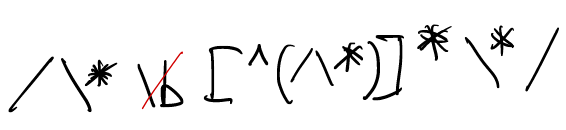
\includegraphics[width=\columnwidth]{img/cregex.png}


\section{Pumping Lemma}
Ist es möglich, einen regulären Ausdruck anzugeben, der auf Zeichenketten der folgenden Form passt? Eine solche Zeichenkette soll mit einer Anzahl n von Zeichengruppen 01 beginnen, gefolgt von genau n Zeichen 2.

$$L=\{(01)^n <2^n | n > 0\}$$
1. Annahme: L ist Regulär \\
2. ∃ Es gibt eine Pumping Length von $N$ \\
3. w $01^n 2^n \in L \ \ \ \|w| ≥ 3 $ \\
4. Aufteilung \\
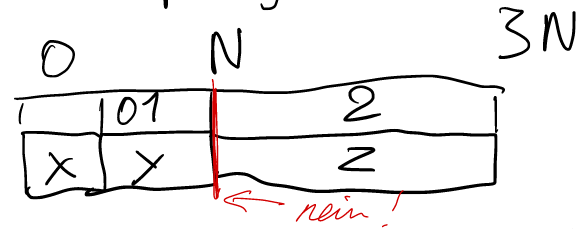
\includegraphics[width=\columnwidth]{img/pumpinglemma.png} \\
(Der OBERE strich zwischen 01 und 2 darf nicht auf Höhe des y strichs sein. Siehe brändli Spick) \\
5. Pumpen: Der y-Teil wird aufgepumpt Anzahl 01 verändert sich, Anzahl 2 bleibt gleich. $xy^k z \notin L$ $∀ k ≠ 2$ \\
6. Widerspruch -> L ist nicht regulär


\section{Pummping Lemma Kontextfrei}

Ein Codierungsverfahren verwendet die Zeichen $\Sigma$ = \{♣, ♢ , ♠ , ♡\} Aus technischen Gründen wird verlangt, dass die Anzahlen der verschiedenen Zeichen in einem Wort sich möglichst nicht unterscheiden, was exakt natürlich nur möglich ist, wenn die Wortlänge durch vier teilbar ist. Für zwei beliebige Zeichen $a,b \in \Sigma$ wird gefordert, dass \\
$$||W|_a - |w|_b| ≤ 1$$
die Anzahlen der Zeichen in einem Wort unterscheiden sich also höchstens um 1. Bei binärer Codierung ist diese Eigenschaft als DC-balance bekannt. Im binären Fall lässt sich DC-balance leicht mit einem Stackautomaten prüfen. Ist dies in diesem Fall mit vier Zeichen auch möglich? \\
$L = {w ∈ \Sigma^∗ | \ ||w|_a −|w|_b|≤ 1 ∀a,b ∈ \Sigma(a ≠ b)}$
1. Wir nehmen an, dass L kontextfrei ist. \\
2. Nach dem Pumping-Lemma für kontextfreie Sprachen gibt es eine Zahl N derart, dass Wörter $w ∈ L$ mit $|w|≥ N$ gepumpt werden.
3. Wir konstruieren das Wort $w = \{♣^N, ♢^N , ♠^N , ♡^N\}$
4. 
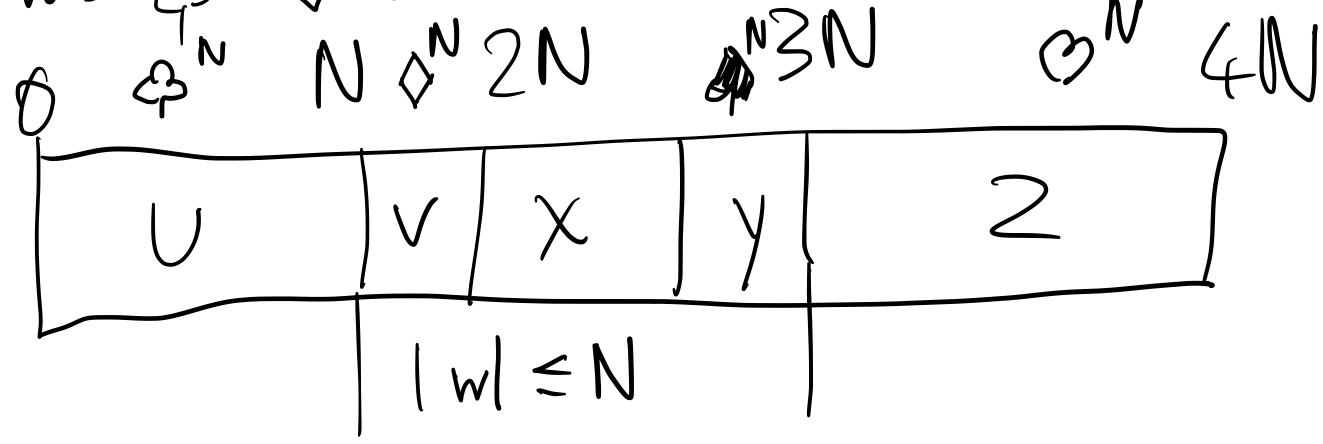
\includegraphics[width=\columnwidth]{img/kontexfreepump.png} \\
5. Beim Pumpen nimmt |♣|, |♢| zu nicht aber |♠| und |♡| $=>$ $ux^k xy^k z \in L | L \forall k ≠ 1$ \\
6. Widerspruch: L ist nicht kontextfrei


\section{How to Solve}
Aufgabentypen Prüfung:\\
1. Reguläre Sprachen (meistens Regex: Spick S. 3)\\
2. Pumping Lemma (Regulär: Spick S. 2, kontextfrei: Spick S. 6)\\
3. Verifizieren (Spick S. 9)\\
4. Satz von Rice/Halteproblem (Spick beides S. 9)\\
5. Grammatik (Spick S. 4/5)\\
6. Grammatik/Pumping Lemma (Spick S. 4/5 oder Regulär: Spick S. 2, kontextfrei: Spick S. 6)\\
7. Karp Problem (Spick S. 12-14)\\
8. Turing-Maschine (Spick S. 6-8)\\
\end{multicols*}
\end{document}